\documentclass[a4paper,12pt]{report}
\usepackage[utf8]{inputenc}


\usepackage{tikz}
\usetikzlibrary{calc}
\usepackage{subcaption}

\begin{document}

\thispagestyle{empty}

\begin{figure}[h!]
		\centering
		\begin{subfigure}{0.5\textwidth}
		\centering
		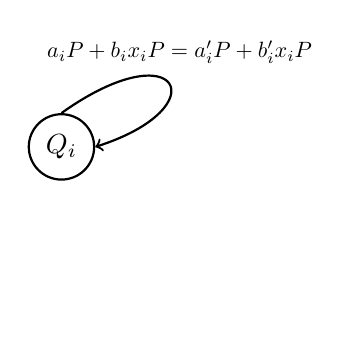
\begin{tikzpicture}
		\node[shape=circle,draw=black,thick] (v) at (0,0) {$Q_i$};
		\node[fill=none] (blank) at (2,-2) {};
        \draw [thick,->] (v.90) .. controls (1.5,1.5) and (2,0.5) .. (v.0);
        \node[scale=0.8] at (1.5,1.2) {$a_iP+b_ix_iP=a'_iP+b'_ix_iP$};
	
		\end{tikzpicture}
		\caption{Cycle of length 1.}
		\end{subfigure}%
		\hfill
		\begin{subfigure}{0.5\textwidth}
		\centering
		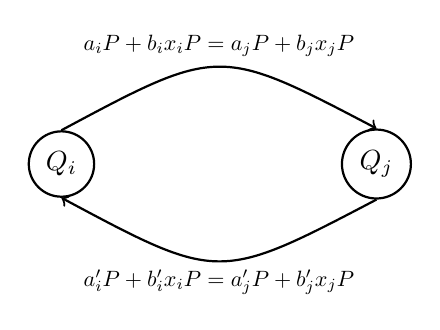
\begin{tikzpicture}
		\node[shape=circle,draw=black,thick] (v) at (0,0) {$Q_i$};
		\node[shape=circle,draw=black,thick] (u) at (4,0) {$Q_j$};
        \draw [thick,->] (v.90) .. controls (2,1.5) .. (u.90);
        \draw [thick,<-] (v.270) .. controls (2,-1.5) .. (u.270);
        \node[scale=0.8] at (2,1.5) {$a_iP+b_ix_iP=a_jP+b_jx_jP$};
        \node[scale=0.8] at (2,-1.5) {$a'_iP+b'_ix_iP=a'_jP+b'_jx_jP$};
	
		\end{tikzpicture}
		\caption{Cycle of length 2.}
		\end{subfigure}
		\caption{Examples of cycles and their corresponding linear systems.}
		\label{fig:MU-lin-sys}
	\end{figure}
\end{document}
